\chapter{Das Registrierungsformular}

Der wohl komplizierteste Teil dieser Diplomarbeit ist der Aufbau und die korrekte Validierung des Registrierungsformulars. Das Ziel ist den Benutzern eine möglichst einfache und schnelle Registrierung, unter Berücksichtigung des derzeitigen Standorts und der dazugehörigen Benutzergruppe, anzubieten. Dafür wurde ein Algorithmus entwickelt, welcher bei der \texttt{ngAfterViewInit()}-Lifecycle-Hook-Methode im \texttt{UserprofileCompo-\\nent} seinen Start nimmt.

\section{Der Algorithmus hinter dem dynamischen Aufbau}

\begin{figure}[H]
	\centerline{
		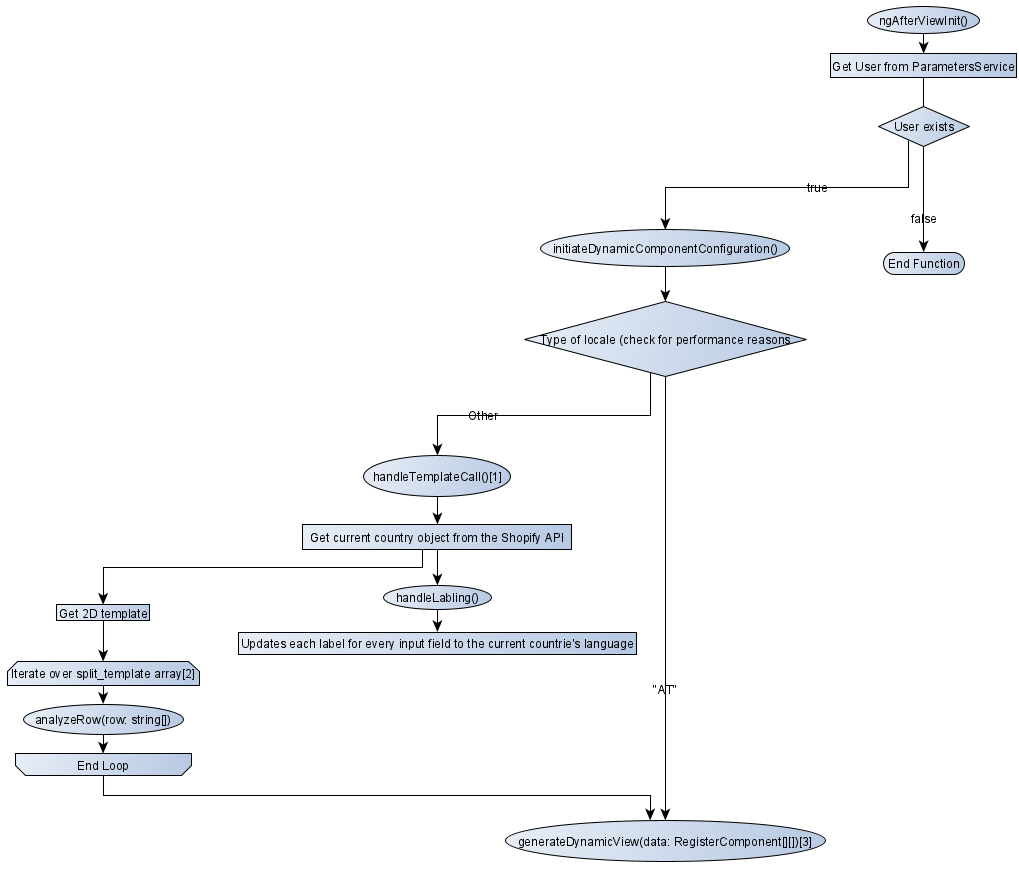
\includegraphics[width=1\textwidth, frame]{./grafiken/RF_Flussdiagramm.png}
	}
	\vskip0pt
	\caption{Flussdiagramm des Algorithmus}
	\label{fig:fc}
\end{figure}

\subsection{\texttt{initiateDynamicComponentConfiguration()}} \label{ssec:lblInitDCC}

Wenn das User-Objekt, welches von der Backend-API abgefragt und erfolgreich als globale Objektvariable gespeichert wurde, wird die \texttt{initiateDynamicComponentConfigu-\\ration()}-Methode aufgerufen. Aus Performance-Gründen basiert die nächste Überprüfung auf dem Wert der aktuellen Lokale. Gleicht dieser den Wert "AT", so wird ein vorgefertigtes Template für ein österreichisches RF, dargestellt im Listing~\ref{lst:template_form_aut}, für die Weiterverwendung benützt. Da davon ausgegangen wird, dass sich vor allem in der Anfangsphase nach der Veröffentlichung hauptsächlich österreichische Kunden ein Konto erstellen, spart dieser Weg enorm viel Zeit, da sofort mit der Erstellung des RF begonnen werden kann.

\begin{lstlisting}[caption={Vordefiniertes Template für das RF}, language=JavaScript,label={lst:template_form_aut}]
export const AUSTRIAN_PRIVATE_PERSON_FORM_Template = [
	[{ type: GenderComponent }],
	[
		{ type: FirstnameComponent, options: { label: "Vorname" } },
		{ type: LastnameComponent, options: { label: "Nachname" } },
	],
	[{ type: StreetComponent, options: { label: "Straße und Hausnummer" } }],
	[
		{ type: CityComponent, options: { label: "Stadt" } },
		{ type: PostalcodeComponent, options: { label: "Postleitzahl" } },
	],
	[
	{
		type: PhoneComponent,
		options: { label: "Telefonnummer", phonePrefix: 43 },
	},
	{ type: DateofbirthComponent },
	],
];
\end{lstlisting}

\subsection{\texttt{handleTemplateCall()}}

Anderenfalls wird als nächster Schritt die \texttt{handleTemplateCall()}-Methode, markiert im Flussdiagramm~\ref{fig:fc} mit [1], aufgerufen, welche, basierend auf dem Wert der aktuellen Lokale, auf die Shopify-API zugreift, um ein \texttt{Country}-Objekt abzurufen. Wurde diese Operation beendet, folgt ein Update auf eine Map, welche vorläufig die Labels für die Wrapper-Objekte speichert. Nachdem das Template geladen wurde, wird über jedes einzelne Element iteriert, markiert im Flussdiagramm~\ref{fig:fc} mit [2], um daraus eine oder mehrere Zeilen zu generieren. Anschließend werden diese in ein 2D-Array gespeichert, welches dann der \texttt{generateDynamicView()}-Methode zur Generierung des RF übergeben wird.

\subsection{\texttt{analyzeRow()}} \label{ssec:lblAnalyzeRow}

\begin{lstlisting}[caption={Erstellung des 2D-Arrays für den Aufbau des RF}, language=JavaScript,label={lst:analyzeRow}]
private analyzeRow(row: string[]): RegisterComponent[][] {
	let addGenderC = false;
	let result: RegisterComponent[][] = [];
	let componentRow: RegisterComponent[] = [];
	
	for (let i = 0; i < row.length; i++) {
		let rowEl = row[i];
		
		if (!addGenderC) {
			if (rowEl.includes("firstName") || rowEl.includes("lastName")) {
				let genderComponent: RegisterComponent[] = [
				{ type: GenderComponent },
				];
				result.push(genderComponent);
				addGenderC = true;
			}
		}
		
		if (rowEl.includes("company") && this.user.isPrivatePerson) {
			break;
		}
		
		for (const x of this.valueMap.keys()) {
			if (rowEl.includes(x)) {
				let compEl: RegisterComponent = {
					type: this.valueMap.get(x),
				};
				
				if (
				compEl.type.prototype ===
				ZoneComponent.prototype
				) {
					compEl.options.zones = this.countryFromService.zones.map(
					(x) => x.name
					);
					this.user.zone = compEl.options.zones[0];
				}
				
				if (
				compEl.type.prototype ===
				PhoneComponent.prototype
				) {
					compEl.options.phonePrefix = this.countryFromService
						.phoneNumberPrefix;
				}
				
				if (this.labels.get(x)) {
					compEl.options.label = this.labels.get(x);
				}
				
				componentRow.push(compEl);
				if (rowEl.includes("phone")) {
					let dateofbirthComponent: RegisterComponent = {
						type: DateofbirthComponent,
					};
					componentRow.push(dateofbirthComponent);
				}
				break;
			}
		}
	}
	result.push(componentRow);
	return result;
}
\end{lstlisting}

Die im Listing~\ref{lst:analyzeRow} beschriebene \texttt{analyzeRow()}-Methode nimmt ein Array von Zeichenfolgen als Parameter und gibt ein 2D-Array von \texttt{RegisterComponent}-Wrapper-Objekten zurück. Obwohl nur eine Reihe aus dem Template, also z. B. \texttt{[\{firstName\} \{lastname\}]}, überprüft wird, kann es wie in diesem Fall sein, dass ein Input zusätzlich darüber erzeugt werden muss. So wird in Zeile neun überprüft, ob der \texttt{GenderComponent} schon hinzugefügt wurde. Trifft das und die Überprüfung, ob in diesem Durchgang der \texttt{FirstnameComponent} oder der \texttt{LastnameComponent} erzeugt werden, wird der \texttt{GenderComponent} als erster eingefügt. Dieser ist für die Auswahl der Anrede zuständig. 

Der selbe Mechanismus kann auch in Zeile 51 gefunden werden, wo es nötig ist, den \texttt{DateofbirthComponent}, welcher für die Eingabe des Geburtstages verantwortlich ist, neben dem \texttt{PhoneComponent} zu generieren.

Anschließend wird in Zeile 19 sicher gestellt, dass eine Privatperson keine Auswahl einer Firma präsentiert wird.

Um nun tatsächlich aus dem Template Objekte zu erzeugen, wird ab Zeile 23 über Schlüssel einer Map, beschrieben im Listing~\ref{lst:valueMap}, welche den String eines Templates als \texttt{key} und den korrespondierenden Component-Objekten als \texttt{value} hat, iteriert. 

\begin{lstlisting}[caption={valueMap in der \texttt{analyzeRow()}-Methode}, language=JavaScript,label={lst:valueMap}]
export class ValueMapper {
	static COMPONENT_VALUE_MAP: Map<string, Type<any>> = new Map();
	
	static COMPONENT_VALUE_MAPPER(){
		this.COMPONENT_VALUE_MAP.set('firstname', FirstnameComponent);
		this.COMPONENT_VALUE_MAP.set('lastname', LastnameComponent);
		this.COMPONENT_VALUE_MAP.set('company', BusinessNameComponent);
		this.COMPONENT_VALUE_MAP.set('address1', StreetComponent);
		this.COMPONENT_VALUE_MAP.set('zip', PostalcodeComponent);
		this.COMPONENT_VALUE_MAP.set('city', CityComponent);
		this.COMPONENT_VALUE_MAP.set('phone', PhoneComponent);
		this.COMPONENT_VALUE_MAP.set('dateOfBirth', DateofbirthComponent);
		this.COMPONENT_VALUE_MAP.set('gender', GenderComponent);
		this.COMPONENT_VALUE_MAP.set('zone', ZoneComponent);
		this.COMPONENT_VALUE_MAP.set('province', ZoneComponent);
		this.COMPONENT_VALUE_MAP.set('state', ZoneComponent);
		return ValueMapper.COMPONENT_VALUE_MAP;
	}
}
\end{lstlisting}

Im ersten Schritt wird, wenn das vom Template angeforderte Feld in der Map existiert, das Wrapper-Objekt erzeugt. 

Wenn dieses den Typ \texttt{ZoneComponent} besitzt, handelt es sich um ein RF, welches für ein Land wie Italien oder Amerika bestimmt ist. Um eine erfolgreiche Registrierung in diesen Ländern abzuschließen, muss hier nämlich die zugehörige Provinz (IT) oder der zugehöriger Bundesstaat (US) angegeben werden. Natürlich funktioniert das für jedes Land, welches dieses Kriterium erfüllen muss. Diese Daten werden anschließend aus dem \texttt{Country}-Objekt der Shopify-API gelesen und als \texttt{zone}-Property in die \texttt{options} gespeichert. 

Im Anschluss wird ebenfalls von diesem Objekt die Telefonnummernvorwahl in die \texttt{options} als \texttt{phoneNumberPrefix}-Property der Wrapper-Klasse gespeichert.

Als letzter Schritt in dieser Methode werden von Zeile 46 bis 48 die Labels, welche vorher in einer Map gespeichert wurden, als \texttt{label}-Property in die \texttt{options} der Wrapper-Objekte gespeichert. 

Nach dem Abschluss wird das Ergebnis an die Schleife der \texttt{initiateDynamicComponent-\\Configuration()}-Methode geliefert und als Zwischenergebnis gespeichert. Wenn die Iteration fertig ist, werden die Zwischenergebnisse zusammengefasst und an die nächste Methode übergeben.

\begin{figure}[H]
	\centerline{
		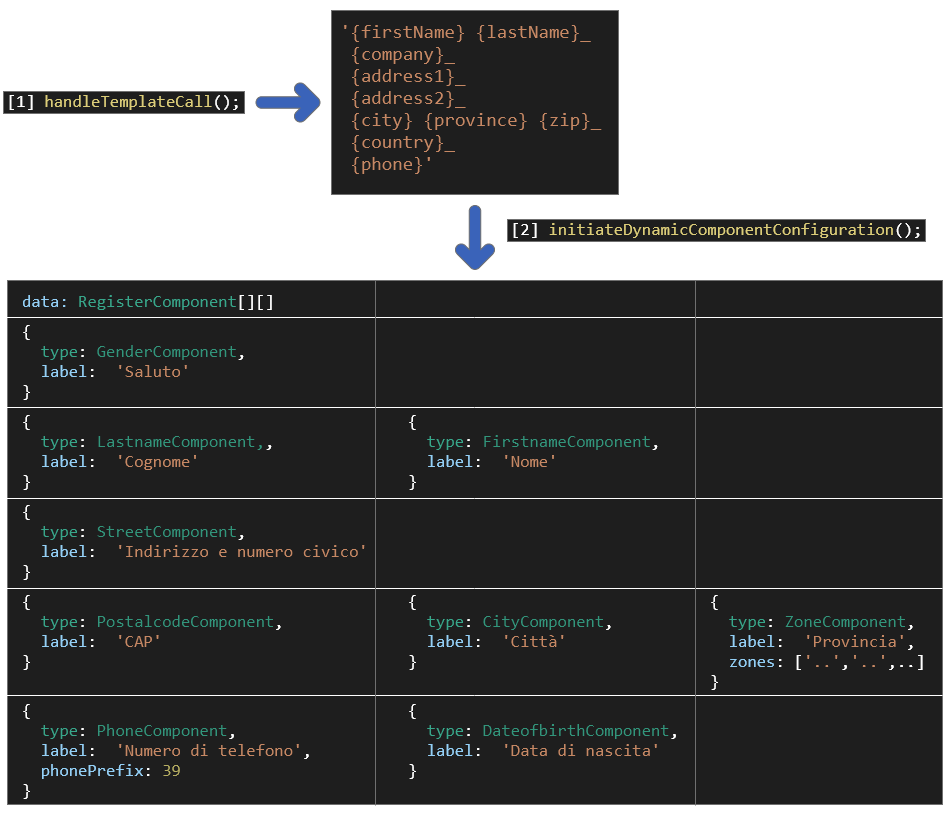
\includegraphics[width=1\textwidth, frame]{./grafiken/RF_Visualisierter Ablauf_1.png}
	}
	\vskip0pt
	\caption{Visualisierter Datenfluss vom Template bis zur Erstellung des 2D-Arrays}
\end{figure}

\subsection{\texttt{generateDynamicView(data: RegisterComponent[][])}}

\begin{lstlisting}[caption={Die \texttt{generateDynamicView()}-Methode}, language=JavaScript,label={lst:generateDynamicView}]
generateDynamicView(data: RegisterComponent[][]) {
for (const element of data) {
	const factory = this.componentFactoryResolver.
	resolveComponentFactory(AutoRowComponentGenerator);
	
	const ref = this.viewContainerRef.createComponent(factory);
	(<AutoRowComponentGenerator>ref.instance).data = element;
	ref.changeDetectorRef.detectChanges();
}
this.bindUserDataToViewData();
}
\end{lstlisting}

Die \texttt{generateDynamicView()}-Methode, markiert im Flussdiagramm~\ref{fig:fc} mit [3], iteriert über jedes Array, um eine \texttt{AutoRowComponentGenerator}-Klasse zu erzeugen. Aus jedem Array in dem 2D-Array wird also eine eigene Reihe für das RF erzeugt. Dabei wird die von Angular bereitgestellte \texttt{ComponentFactoryResolver}-Klasse verwendet, um aus einer Klasse einen Component zu erstellen. 
Jede Reihe, also jeder \texttt{AutoRowComponent-\\Generator}, wird dann nacheinander in die HTML-Datei durch eine \texttt{ViewContainerRef} eingefügt. Die \texttt{ViewContainerRef} verweist auf ein HTML-Element, wie es das Listing~\ref{lst:html} beschreibt.

\begin{lstlisting}[caption={ViewContainerRef verweist auf \#componentHook}, language=JavaScript,label={lst:html}]
<form #dynamicForm>
	<div #componentHook></div>
</form>
\end{lstlisting}

Das Array aus Wrapper-Klassen wird anschließend dem erzeugten Component als \texttt{data}-Objekt übergeben. \texttt{detectChanges()} sagt dem Component, dass er die Lifecycle-Hook-Methode \texttt{ngAfterViewInit()} erneut aufrufen muss. Wie im Listing~\ref{lst:nginARCG} erklärt wird, ist diese dafür verantwortlich, dass die übergebenen Daten verarbeitet werden.

Da das RF in der Profilübersicht wieder verwendet wird, ist es wichtig, die Daten, welche vom Benutzer bereits vorhanden sind, in das frisch erstellte RF durch die Methode \texttt{bindUserDataToViewData()} wieder einzubinden.

\subsection{Die \texttt{AutoRowComponentGenerator}-Klasse}

\begin{lstlisting}[caption={Die \texttt{ngAfterViewInit()}-Methode der \texttt{AutoRowComponentGenerator}-Klasse}, language=JavaScript,label={lst:nginARCG}]
ngAfterViewInit(): void {
	for (const x of this.data) {
		const factory = this.componentFactoryResolver
		.resolveComponentFactory(x.type);
		
		const ref = this.viewContainerRef.createComponent(factory);
		this.checkComponentRef(ref, x);
		ref.changeDetectorRef.detectChanges();
	}
	this.addClasses();
}
\end{lstlisting}

Anders als bei der \texttt{generateDynamicView()}-Methode wird nicht über ein 2D-Array iteriert, um ein Array an Daten zu übergeben, sondern über das tatsächliche Array, welches eine Reihe aus Feldern repräsentiert. Diese werden dann nach der Reihe auf die selbe Weise erzeugt. \texttt{checkComponentRef()} bindet die \texttt{options} der Wrapper-Klasse an die erzeugten Components, wie im Listing~\ref{lst:ccr} gezeigt wird. So ist es nun möglich, das RF dynamisch zur Laufzeit zu Erzeugen und in der UI anzuzeigen.

\begin{lstlisting}[caption={Die \texttt{checkComponentRef()}-Methode der \texttt{AutoRowComponentGenerator}-Klasse}, language=JavaScript,label={lst:ccr}]
checkComponentRef(ref: ComponentRef<any>, component: RegisterComponent) {
	if (component.options) {
		if (component.options.zones) {
			(ref.instance as ZoneComponent).zones = component.options.zones;
		}
		
		if (component.options.label) {
			(ref.instance as ComponentValueConfigurator).setLabel(
			component.options.label
			);
		}
		
		if (component.options.phonePrefix) {
			(ref.instance as PhoneComponent).setPhonePrefix(
			component.options.phonePrefix
			);
		}
	}
}
\end{lstlisting}

Abschließend werden noch CSS-Klassen für bestimmte Komponenten vergeben.

\begin{figure}[H]
	\centerline{
		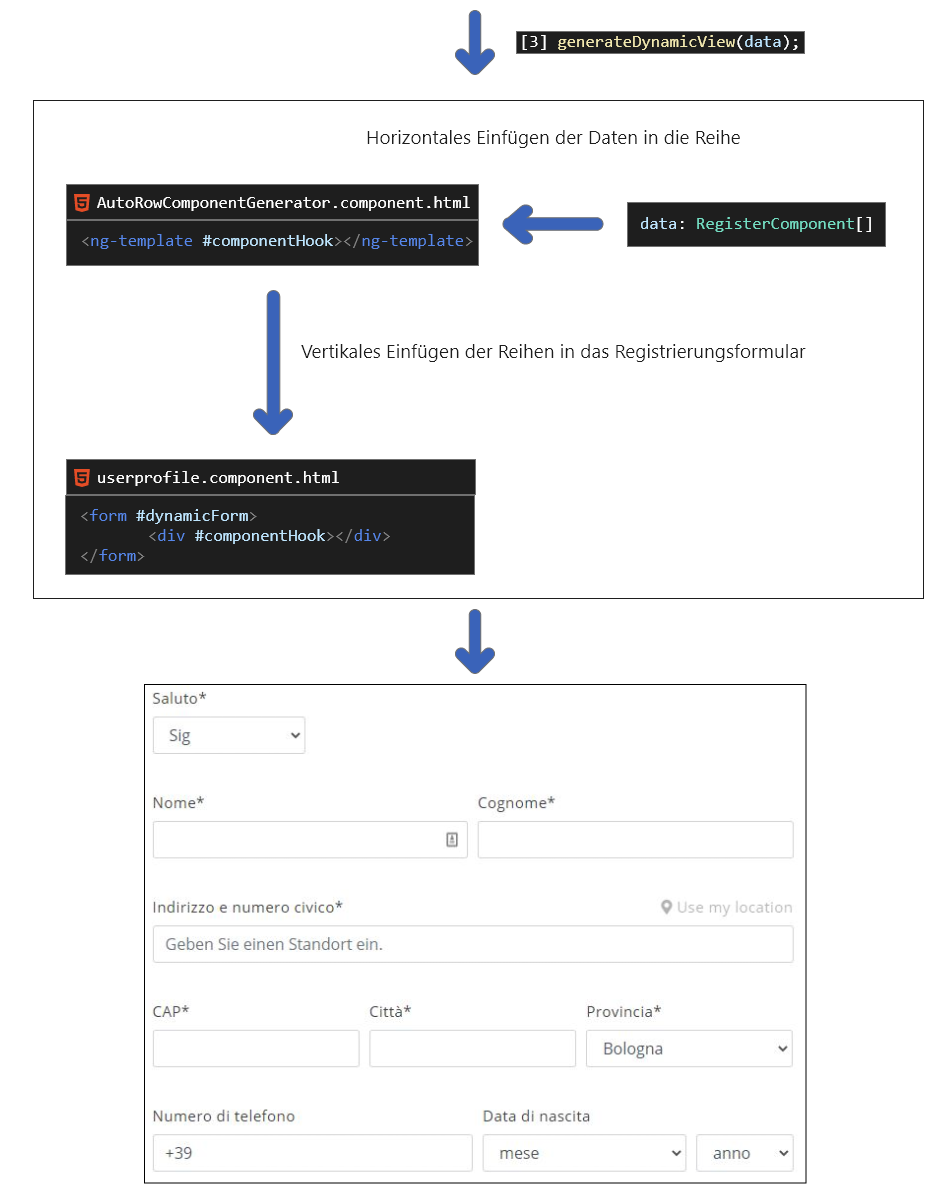
\includegraphics[width=1\textwidth, frame]{./grafiken/RF_Visualisierter Ablauf_2.png}
	}
	\vskip0pt
	\caption{Visualisierter Datenfluss vom 2D-Array bis zum fertigen RF}
\end{figure}

\section{Die Validierungsmethodik}
\subsection{Allgemeines}

Für eine effiziente und dynamische Validierung wurde der \texttt{ValidatorService} programmiert. Grundsätzlich implementiert jeder Component, welcher im Registrierungsformular erzeugt wird, das \texttt{ComponentValueConfigurator}-Interface. Dadurch wird gewährleistet, dass der \texttt{ValidatorService} auf die im Listing~\ref{lst:edic} verwiesenen Methoden zugriff erhält.

\begin{lstlisting}[caption={Methoden aus dem \texttt{ComponentValueConfigurator}-Interface}, language=JavaScript,label={lst:edic}]
export declare interface ComponentValueConfigurator{
	setLabel(label: string): void;
	onFocusChange(event: any);
	validateInput();
}
\end{lstlisting}

Wie man erkennen kann, wird die \texttt{setLabel()}-Methode im Listing~\ref{lst:ccr} dazu benötigt, um jeden Component sein Label zu übergeben.

Im \texttt{ValidatorService} wird beim Initialisieren eine Map mit einem \texttt{string} als Key und einem \texttt{Options}-Objekt als Value erstellt. Diese wird über ein \texttt{BehaviorSubject<Map\\<string, Options>>} an alle Observer verteilt.

\begin{lstlisting}[caption={Die \texttt{fields}-Map und ihr Subject}, language=JavaScript]
	private fields: Map<string, Options> = new Map<string,Options>();
	private fieldsSub = new BehaviorSubject<Map<string, Options>>(this.fields);
\end{lstlisting}

Wie im Listing~\ref{lst:opvasta} gezeigt wird, beinhaltet das \texttt{Options}-Objekt alle wichtigen Variablen, welche im weiteren Verlauf für die Validierung benötigt werden.

\begin{lstlisting}[caption={Das \texttt{Options}-Objekt und seine abhängigen Objekte}, language=JavaScript,label={lst:opvasta}]
export interface Options {
	state: State;
	validators?: ValidatorManager[];
	value?: any;
}
export interface ValidatorManager{
	validator: (value: any) => boolean;
	errorMessage: string;
}
export interface State {
	isValid: boolean;
	isTouched: boolean;
	isPrestine: boolean;
	isNotRequired?: boolean;
}
\end{lstlisting}

\subsection{Validierung am Beispiel des \texttt{FirstnameComponent}}
\subsubsection{Die Initialisierung}
Wird ein Component erstellt, registriert sich dieser in der \texttt{ngOnInit()}-Lifecycle-Hook-Methode sofort in der \texttt{fields}-Map. Seine übergebenen Werte werden an alle Observer, wie unter anderem der \texttt{UserprofileComponent}, verteilt. 

\begin{lstlisting}[caption={Der Konstruktor und die \texttt{ngOnInit()}-Lifecycle-Hook-Methode des \texttt{FirstnameComponent}}, language=JavaScript]
constructor(public validatorService: ValidatorService) {
	validatorService
	.getFieldsObservable()
	.subscribe((x) => (this.fields = x));
}

ngOnInit(): void {
	const state = { isValid: false, isTouched: false, isPrestine: true };
	const validators = [
	{
		validator: (value: string) => value != null,
		errorMessage: "ValidationError.FirstnameUnset",
	},
	{
		validator: (value: string) => value.length >= 2,
		errorMessage: "ValidationError.FirstnameTooShort",
	},
	];
	
	this.validatorService.addFields('firstName', {
		state: state,
		validators: validators,
	});
}
\end{lstlisting}

Im Konstruktor hängt sich der \texttt{FirstnameComponent} auf das \texttt{fieldsSub - BehaviorSubject} als Observer und erhält somit immer die aktuellsten Daten. Die Daten, welche übergeben werden, können wie folgt zusammengefasst werden:

\begin{itemize}
	
	\item \texttt{state}: Der Zustand des aktuellen Eingabefelds:
		\begin{itemize}
			\item	\texttt{isValid}: boolean => Eingabefeld wurde erfolgreich validiert.
			\item	\texttt{isTouched}: boolean => Der Benutzer hat das Eingabefeld bereits besucht.
			\item	\texttt{isPrestine}: boolean => Der Benutzer hat das Eingabefeld bereits verwendet und Werte verändert.
			\item	\texttt{isNotRequired?}: boolean => Das Eingabefeld wird nicht für eine erfolgreiche Validierung benötigt (z. B. die Eingabe des Geburtstages).
		\end{itemize}
	\item \texttt{validators}: Dieses Objekt ist ein Array aus \texttt{ValidatorManager}-Objekten. Einem \texttt{ValidatorManager}-Objekt wird eine Callback-Methode übergeben, welche mit der Aufgabe des Validierens beauftragt ist. Anschließend wird noch ein Key für eine Fehlermeldung mitgegeben, welche angezeigt wird, wenn der Validator fehl schlägt. 
\end{itemize}

\subsubsection{Die HTML-Datei}

\begin{lstlisting}[caption={Der HTML-Datei des \texttt{FirstnameComponent}}, language=JavaScript]
<label for="inputFirstname">{{ label }}*</label>

<input id="inputFirstname" name="inputFirstname" type="text" class="form-control" autocomplete="fname" [(ngModel)]="fields.get(key).value" (change)="validatorService.inputChanged(key)" (focus)="onFocusChange($event)" (focusout)="onFocusChange($event)"/>

<small class="text-danger" *ngIf="!fields.get(key).state.isValid && !fields.get(key).state.isPrestine">{{ errorMessage | translate}}</small>
\end{lstlisting}

Im Prinzip unterscheiden sich die HTML-Dateien der verschiedenen Komponenten kaum und besteht aus folgenden Elementen:

\begin{itemize}
	\item Das \texttt{input}-Element kümmert sich um die Benutzereingaben. Abhängig davon, welche Aktion der Benutzer ausführt, werden verschiedene Events ausgeführt:
	
		\begin{itemize}
			\item \texttt{[(ngModel)]}: Synchronisiert den Wert der Eingabe mit der verwiesenen Variable. Die Synchronisation erfolgt hierbei auf beiden Wegen. Wird der Wert im Eingabefeld geändert, wird auch der Wert der Variable geändert. Wird aber der Wert der Variable, z. B. durch das manuelle Setzten des Wertes in der \texttt{bindUserDataToViewData()}-Methode, zu finden in Zeile zehn im Listing~\ref{lst:generateDynamicView}, geändert, wird der neue Wert auch so auch auf der Website angezeigt. 
			
			\item \texttt{(change)}: Das \texttt{change}-Event wird getriggert, wenn sich der Wert der Variable ändert. Daraufhin wird der Wert \texttt{isPrestine} für dieses Feld auf \texttt{false} gesetzt, da es sich nicht mehr um ein sauberes Eingabefeld handelt.
			
			\item \texttt{(focus) / (focusout)}:  Sollte der Benutzer das Eingabefeld betreten oder verlassen, wird der  Wert \texttt{isTouched} auf \texttt{true} gesetzt. Solle es sich um das \texttt{(focusout)}-Event handeln, wird die im Listing~\ref{lst:validateInput} beschriebene \texttt{validate-\\Input()}-Methode aufgerufen.
		\end{itemize} 
	
	\item Das \texttt{small}-Element repräsentiert die anzuzeigende Fehlermeldung. Diese wird nur dann angezeigt, wenn der Wert \texttt{isValid} der verwiesenen Variable \texttt{false} ist und diese auch tatsächlich verändert wurde. 
\end{itemize}

\subsubsection{Der Validierungsprozess}

Also jedes mal, wenn der Benutzer des Eingabeelement verlässt, wird dieses auch validiert. Wie auch schon bei der HTML-Datei unterscheidet sich diese Methode kaum unter den Komponenten.

\begin{lstlisting}[caption={Die Validierung innerhalb Komponenten}, language=JavaScript,label={lst:validateInput}]
validateInput() {
	const validators =  this.fields.get(this.key).validators;
	const currentVal = this.fields.get(this.key).value;
	
	for (let i = 0; i < validators.length; i++) {
		const validator = validators[i];
		if (!validator.validator(currentVal)) {
			
			this.errorMessage = validator.errorMessage;
			this.fields.get(this.key).state.isValid = false;
			this.validatorService.emitFormValidation();
			return;
		}
	}
	this.fields.get(this.key).state.isValid = true;
	this.validatorService.emitFormValidation();
}
\end{lstlisting}

Ab Zeile sechs wird über jeden Validator iteriert, um anschließend die Callback-Methoden aufzurufen. Glückt jede Überprüfung, wird die \texttt{isValid}-Variable auf \texttt{true} gesetzt. 

Scheitern diese Überprüfungen jedoch, wird die Fehlermeldung aus dem Validator-Objekt gelesen und in eine globale Variable gespeichert. Da nun die Werte der Variablen \texttt{isValid} und \texttt{isPrestine} jeweils dem Wert \texttt{false} entsprechen, wird die Fehlermeldung angezeigt. 

In beiden Fällen wird die im \texttt{ValidatorService} implementierte \texttt{emitFormValidation()}-Methode, beschrieben im Listing~\ref{lst:emitFormValidation}, aufgerufen.

\begin{lstlisting}[caption={Die Validierung aller Komponenten im \texttt{ValidatorService}}, language=JavaScript,label={lst:emitFormValidation}]
emitFormValidation() {
	if (this.fields.values) {
		for (const option of this.fields.values()) {
			if (!option.state.isValid) {
				if (!option.state.isNotRequired) {
					this.formIsValid = false;
					this.formIsValidSub.next(this.formIsValid);
					return;
				}
			}
		}
		this.formIsValid = true;
		this.formIsValidSub.next(this.formIsValid);
	} else {
		this.formIsValid = false;
		this.formIsValidSub.next(this.formIsValid);
	}
}
\end{lstlisting}

Diese Methode iteriert über alle \texttt{Options}-Objekte der \texttt{fields}-Map. Entspricht der Wert der Variable \texttt{isValid} bei allen Objekten \texttt{true}, so wird das Boolean-Objekt \texttt{formIsValid} durch ein Subjekt an alle Observer verschickt.

Der \texttt{UserprofileComponent} benützt diese Variable um, wie im Listing~\ref{lst:btn} gezeigt wird, den Button, welcher beim Drücken alle Werte der \texttt{fields}-Map ausliest, in das aktuelle Benutzerobjekt speichert und dieses zum Backend schickt, basierend auf dem Wert der Variable zu de- oder aktivieren.

\begin{lstlisting}[caption={Der Button im \texttt{UserprofileComponent}, welcher de- oder aktiviert wird}, language=JavaScript,label={lst:btn}]
<button 
	[disabled]="!formIsValid" 
	(click)="onBtnClick()" 
	type="submit"
	class="btn btn-poettinger"
	>{{buttonLabel}}
</button>
\end{lstlisting}

\begin{figure}[H]
	\centering
	\subfloat[][]{
		
\includegraphics[width=0.3\textwidth]{./grafiken/rf_unvalid_button.PNG}
	}
	\qquad
	\subfloat[][]{
		
\includegraphics[width=0.3\textwidth]{./grafiken/rf_valid_button.PNG}
	}
	\caption{(a): Deaktivierter Button im RF, (b): Aktivierter Button im RF}%
\end{figure}

\section{Die Komfortfunktionen}
Die Komfortfunktionen wurden implementiert, um es den Benutzern so einfach wie möglich zu machen und ohne viel Aufwand alle Daten eingeben zu können.
\subsection{Automatische Adressvervollständigungsvorschläge}
\subsubsection{Der Google-API-Key}
Um auf die Google-API zugriff zu erhalten, wurde ein Google-API-Key erzeugt. Dieser wird aus folgenden Gründen erst bei der Verwendung im \texttt{AutocompleteComponent} geladen:

\begin{itemize}
	
	\item Sicherheit: Der API-Key wird nur dann als \texttt{script}-Element in den HTML-Head geladen, wenn dieser auch zur Verwendung gebraucht wird. Das dient dazu, dass der API-Key nicht sofort bei Hackerattacken oder von Webcrawler ausgelesen werden kann.
	
	\item Geschwindigkeit: Da diese Google-JS-Library keine Tree-Shakable-Library ist, sprich, man muss die komplette Bibliothek an Funktionen importieren, ist das Laden sehr zeitaufwändig. Je mehr \texttt{script}-Elemente im HTML-Head geladen werden, umso langsamer ladet die Website beim Aufruf.
	
	\item Preis: Je öfter der API-Key als \texttt{script}-Elemente im HTML-Head geladen wird, umso öfter wird von Google ein Preis für die Benutzung verrechnet.
\end{itemize}

Der API-Key wird über eine Direktive eines HTML-Elements in den HTML-Head geladen:

\begin{lstlisting}[caption={Die \texttt{ngOnInit()}-Methode der \texttt{LoadScriptDirective}}, language=JavaScript,label={lst:gpac}]
ngOnInit() {
	let node = document.createElement('script');
	node.src = this.param;
	node.type = 'text/javascript';
	node.async = false;
	let keyExists = false;
	let head = document.getElementsByTagName('head')[0];
	head.childNodes.forEach(x => {
		if (x.isEqualNode(node)) {
			keyExists = true;
		}
	});
	if (!keyExists) {
		head.appendChild(node);
	}
}
\end{lstlisting}

Der, auf in Zeile drei verwiesene \texttt{this.param,} ist ein \texttt{@Input('script')}-Element, welches der API-Key übergeben wird. Wenn die \texttt{LoadScriptDirective} nicht mehr aktiv ist, wird das \texttt{script}-Element wieder aus dem DOM entfernt.

\subsubsection{Implementierung}
Die automatischen Adressvervollständigungsvorschläge kommen beim Laden des \texttt{Street-\\Component} zum Einsatz. Wenn der Benutzer im Feld \texttt{Straße und Hausnummer*} anfängt seine Adresse einzutippen, werden ihm automatische Vorschläge, basierend auf dem aktuell ausgewähltem Land, von der API präsentiert. 

\begin{figure}[H]
	\centerline{
		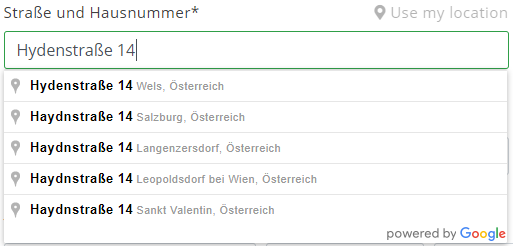
\includegraphics[width=1\textwidth, frame]{./grafiken/open_adress_completion.PNG}
	}
	\vskip0pt
	\caption{Automatisch generierte Adressvervollständigungsvorschläge in Österreich}
\end{figure}

\begin{figure}[H]
	\centerline{
		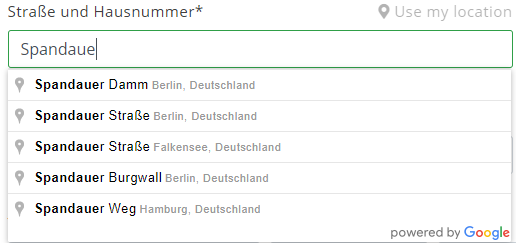
\includegraphics[width=1\textwidth, frame]{./grafiken/open_adress_completion_de.PNG}
	}
	\vskip0pt
	\caption{Automatisch generierte Adressvervollständigungsvorschläge in Deutschland}
\end{figure}

Dafür wurde eine Hierarchieebene darunter ein weiterer Komponent, der \texttt{Autocomplete-\\Component} eingebaut, welcher ein HTML-Input-Element mit der Direktive \texttt{\#addresstext} besitzt. Mithilfe des in Angular integriertem \texttt{@ViewChild('..')-Property decorator} ist es nun möglich, eine globales Objekt aus dem HTML-Input-Element zu erzeugen. 

\begin{lstlisting}[caption={Die \texttt{getPlaceAutocomplete()}-Methode der \texttt{AutocompleteComponent}-Klasse}, language=JavaScript,label={lst:gpac}]
getPlaceAutocomplete() {
	const autocomplete = new google.maps.places.Autocomplete(
	this.addresstext.nativeElement,
	{
		types: ['address']
	});
	
	google.maps.event.addListener(autocomplete, 'place_changed', () => {
		const place = autocomplete.getPlace();
		this.setAddress.emit(place);
	});
}
\end{lstlisting}

Wie im Listing~\ref{lst:gpac} ersichtlich ist, wird das Objekt anschließend dazu verwendet, um ein \texttt{google.maps.places.Autocomplete}-Objekt, welches als Parameter die zu generierenden Vorschläge übergeben wird, zu erzeugen. In diesem Fall wird dem Objekt gesagt, nur Adressvorschläge zu generieren. Auf dieses wird dann ein \texttt{place\_changed}-Event registriert. Wird das Event getriggert, feuert ebenfalls der \texttt{setAddress-\\EventEmitter} und liefert somit die übergebenen Daten an alle registrierten Observer.

\begin{lstlisting}[caption={Die \texttt{addressHasBeenSelected()}-Methode der \texttt{StreetComponent}-Klasse}, language=JavaScript,label={lst:gpac}]
addressHasBeenSelected(place: google.maps.places.PlaceResult) {
	let addressDto: AddressDto = {
		city: "",
		countryCode: "",
		postalcode: "",
		street: "",
		streetNumber: "",
	};
	
	place.address_components.forEach((x) => {
		if (x.types.includes("street_number")) {
			addressDto.streetNumber = x.long_name;
		} else if (x.types.includes("route")) {
			addressDto.street = x.long_name;
		} else if (x.types.includes("locality")) {
			addressDto.city = x.long_name;
		} else if (x.types.includes("postal_code")) {
			addressDto.postalcode = x.long_name;
		} else if (x.types.includes("country")) {
			addressDto.countryCode = x.short_name;
		}
	});
	
	this.handleAddressDto(addressDto);
}
\end{lstlisting}

Der \texttt{StreetComponent} hat sich mit der \texttt{addressHasBeenSelected()}-Methode auf dieses Event als Observer registriert. Da das überlieferte Objekt ein Array an Ergebnissen liefert, werden über diese iteriert und die Ergebnisse in ein temporäres Objekt gespeichert. Die \texttt{handleAddressDto()}-Methode aktualisiert jeden Wert in der \texttt{fields}-Map. 

Das interessante daran ist, wenn manuell eine Adresse eines anderen Landes eingegeben wird, ein Event im \texttt{ValidatorService}, auf welches der \texttt{UserprofileComponent} registriert ist, abgefeuert wird. Es wird umgehend die \texttt{onInitViewChange()}-Methode aufgerufen, welche alle Nachfolgenden Elemente des HTML-Form-Elements, zu finden im Listing~\ref{lst:html}, löscht und wieder bei der \texttt{initiateDynamicComponentConfiguration()}-Methode startet. Somit wird ein, für das neue Land angepasste, RF generiert (Kapitel ~\ref{ssec:lblInitDCC}).


\subsection{Ermittlung des Standorts durch die IP - Use my location}

Die Funktion für die automatische Standorterkennung wird durch einen Klick auf "Use my location" ausgelöst. Um auf den tatsächlichen Standort des Benutzers zugriff zu erhalten, muss dieser jedoch davor um seine Erlaubnis gefragt.\autocite{useMyLocation}

Die Standortermittlung funktioniert mit der \texttt{getCurrentPosition()}-Methode des \texttt{navigator.geolocation}-Objektes, welche im Listing \ref{lst:useMyLocation} zu finden ist. Dabei wird eine asynchrone Abfrage gestartet, welche die Position abruft. Bei erfolgreichem Abschluss dieser Abfrage, wird die mitgegebene Funktion mit der gefundene Position ausgeführt. Als optionalen zweiten Parameter kann dabei auch eine Funktion mitgegeben werden, die nur bei Auftreten eines Fehlers aufgerufen wird. \autocite{useMyLocation}

\begin{lstlisting}[caption={Die \texttt{onUseMyLocationClicked()}-Methode der \texttt{StreetComponent}-Klasse}, language=JavaScript,label={lst:useMyLocation}]
onUseMyLocationClicked() {
	navigator.geolocation.getCurrentPosition(pos => this.workWithLocation(pos, this));
}
\end{lstlisting}

Nachdem das Positionsobjekt erfolgreich erhalten wurde, wird die Methode von dem Listing \ref{lst:workWithLocation} aufgerufen. Dabei werden als erstes die Längen- und Breitengrade aus dem Positionsobjekt ausgelesen. Dies geschieht in Zeile zwei und drei des Listings \ref{lst:workWithLocation}. Mittels der Google Maps API werden diese zwei erstellten Variablen in ein LatLng-Objekt umgewandelt.\autocite{latLngObjekt} Den Google Maps Geocoder wird in Zeile fünf dieses LatLng-Objekt und eine Callback-Funktion in die Methode \texttt{geocode()} übergeben. Nach der Überprüfung ob das geocoding erfolgreich war, wird das Ergebnis in ein AddressDto gespeichert. Anschießend darauf wird die Methode \texttt{handleAddressDto()} mit der gespeicherten Adresse aufgerufen, die alle bezogenen Werte der \texttt{fields}-Map aktualisiert.

\begin{lstlisting}[caption={Die \texttt{workWithLocation()}-Methode der \texttt{StreetComponent}-Klasse}, language=JavaScript,label={lst:workWithLocation}]
private workWithLocation(position, self: this) {
	const latitude = position.coords.latitude;
	const longitude = position.coords.longitude;
	let latlng = new google.maps.LatLng(latitude, longitude);
	let geocoder = new google.maps.Geocoder();
	let addressDto: AddressDto = { city: '', countryCode: '', postalcode: '', street: '', streetNumber: '' };
	geocoder.geocode({ location: latlng }, function (results, status) {
		if (status === 'OK') {
			if (results[0]) {
				results[0].address_components.forEach(x => {
					if (x.types.includes('street_number')) {
						addressDto.streetNumber = x.long_name;
					}
					else if (x.types.includes('route')) {
						addressDto.street = x.long_name;
					}
					else if (x.types.includes('locality')) {
						addressDto.city = x.long_name;
					}
					else if (x.types.includes('postal_code')) {
						addressDto.postalcode = x.long_name;
					}
					else if (x.types.includes('country')) {
						addressDto.countryCode = x.short_name;
					}
				});
				self.handleAddressDto(addressDto);
			}
		}
	});
}
\end{lstlisting}

\subsection{Automatische Telefonnummerprefix Erkennung}

Wie im Kapitel~\ref{ssec:lblAnalyzeRow} [\texttt{analyzeRow()}] bereits erklärt wird, wird die Telefonnummernvorwahl aus dem \texttt{Country}-Objekt der Shopify-API gelesen und in die \texttt{options} als \texttt{phoneNumberPrefix}-Property der Wrapper-Klasse gespeichert.